\documentclass[a4paper,12pt,french]{report}
\usepackage{babel} 
\usepackage[T1]{fontenc} 
\usepackage[utf8]{inputenc} 
\usepackage{lmodern}
\usepackage{amsthm}
\usepackage{stmaryrd}
\usepackage{amsmath}
\usepackage{amssymb}
\usepackage{mathrsfs}
\usepackage{geometry}
\usepackage{graphicx}
\usepackage{boiboites}
\geometry{hmargin=2.5cm,vmargin=2cm}
\renewcommand{\qedsymbol}{$\checkmark$}
%\newtheorem{axiome}{Axiome}[section]
\newtheorem{lemma}{Lemme}[section]
%\newtheorem{proposition}{Proposition}[section]
\newtheorem{theorem}{Théorème}[section]
\newtheorem{definition}{Définition}[section]
\newtheorem{exemple}{Éxemple}[section]

% ------

\definecolor{violet}{rgb}{0.5,0,0.5}
\definecolor{orange}{rgb}{0.9,0.4,0}

\newboxedtheorem[boxcolor=blue,titleboxcolor = blue,titlebackground=blue!20,titlecolor = black]{proposition}{Proposition}{subsection}
\newboxedtheorem[boxcolor=red,titleboxcolor = red,titlebackground=red!20,titlecolor = black]{axiome}{Axiome}{part}

% ------


\title{TIPE : Origami et constructibilité}

\begin{document}
\maketitle
\renewcommand{\contentsname}{Sommaire}
\tableofcontents{}

\chapter{Introduction à la constructibilité : règle et compas}
		Il est nécessaire de commencer notre étude en posant quelques définitions et résultats élémentaires qui nous seront utiles par la suite.
		\section{Outils d'algèbre}
			
			\begin{definition}[Corps] 
				Un corps est une structure algébrique \( (\mathbb{K} , + , \times ) \) telle que :
				\begin{enumerate}
					\item Les lois \( + \) et \( \times \) sont des applications \( \mathbb{K}^2 \longrightarrow \mathbb{K} \)
					\item \((\mathbb{K} , +)\) soit un groupe commutatif, c'est-à-dire :
						\[ 
							\left\{ 
							\begin{array}{lll}
								\exists \, 0_{\mathbb{K}} \in \mathbb{K} , \forall x \in \mathbb{K}, x + 0_{\mathbb{K}} = 0_{\mathbb{K}} + x = x
								\\
								\forall x \in \mathbb{K} , \exists k \in \mathbb{K} , x + k = k + x = 0_{\mathbb{K}} \mbox{  et on notera } -x = k
								\\
								\forall (x,y) \in \mathbb{K}^{2},
											x + y = y + x
										
								\\
								\forall (x, y, z) \in \mathbb{K}^3, (x + y) + z = x + (y + z)
									 
							\end{array}
							\right.
						\]
					\item \((\mathbb{K}\setminus\{0\}, \times) \) est un groupe commutatif :
						\[ 
								\left\{ 
								\begin{array}{lll}
									\exists \, 1_{\mathbb{K}} \in \mathbb{K}\setminus\{0\} , \forall x \in \mathbb{K}\setminus\{0\}, x \times 1_{\mathbb{K}} = 1_{\mathbb{K}} \times x = x
									\\
									\forall x \in \mathbb{K}\setminus\{0\} , \exists k \in \mathbb{K}\setminus\{0\} , x \times k = k \times x = 1_{\mathbb{K}} \mbox{  et on notera } x^{-1} = k
									\\
									\forall (x,y) \in (\mathbb{K}\setminus\{0\})^{2},
												x \times y = y \times x
									\\
									\forall (x, y, z) \in (\mathbb{K}\setminus\{0\})^3, (x \times y) \times z = x \times (y + z)
										 
								\end{array}
								\right.
							\]
					\item La loi \( + \) est distributive sur la loi \( \times \) :
						\[
						\forall (x, y, z) \in \mathbb{K}^3, x \times (y + z) = (y + z) \times x = xy + xz
						\]
				\end{enumerate}
			
			\end{definition}
			
			\begin{definition}[Corps engendré]
				Soit \(\mathbb{E}\) et \(\mathbb{F}\) deux corps, tel que \(\mathbb{E} \subset \mathbb{F}\), et soit \(x \in \mathbb{F} \). Le corps engendré par \(x\), noté \(\mathbb{E}(x)\), est le plus petit corps (au sens de l'inclusion) qui contient x et \(\mathbb{E}\).
			\end{definition}
			
			\begin{definition}[Sous anneau engendré par x]
				Soit \(\mathbb{E}\) et \(\mathbb{F}\) deux corps, tels que \(\mathbb{E}\subset\mathbb{F}\), et \(x\in\mathbb{F}\). Alors on appelle \emph{Sous anneau de F engendré par x} l'ensemble :
				\[\left\{y\in F / \exists P \in E[X], y = P(x)\right\}\]
				On le note \(E[x]\).{}
				
				\begin{proof}
					\(E[x]\) est l'image de l'anneau \(E[X]\) par le morphisme d'évaluation \[\varphi_{x} : \; P \mapsto P(x) \] donc c'est un anneau. Par la suite on introduira \(\varphi_{x}\) systématiquement, sans le redéfinir.
				\end{proof}
				
			\end{definition}
			
			
			\begin{definition}[Espace Vectoriel]
				Un \(\mathbb{K}\)-espace vectoriel \(E\)  est une structure algébrique \( (E, + , \cdot)\) telle que
				\begin{enumerate}
					\item \( (E, +) \) est un groupe commutatif
					\item La loi externe \( \cdot \) est une application \( \mathbb{K} \times E \longrightarrow E \) qui vérifie les axiomes suivants :
						\begin{enumerate}
							\item Pseudo-associativité :
								\(
								\forall (\lambda, \mu, x) \in \mathbb{K}^2 \times E, \mu(\lambda x) = (\mu \lambda) x
								\)
							\item Pseudo-distributivité :
								\(
								\left\{
									\begin{array}{ll}
										\forall (\lambda, \mu, x) \in \mathbb{K}^2 \times E , (\lambda + \mu)x = \lambda x + \mu x \\
										\forall (\lambda, x, y) \in \mathbb{K} \times E^2 , \lambda(x + y) = \lambda x + \lambda y
									\end{array}
								\right.
								\)
							\item Opérateur neutre :
								\(
								\forall x \in E, 1_\mathbb{K} \cdot x = x
								\)
						\end{enumerate}
				\end{enumerate}
				
			\end{definition}
			
			
			\begin{definition}[Extension de corps]
			
				Si \( \mathbb{K} \) et \( \mathbb{L} \) sont deux corps tels que \(\mathbb{K} \subset  \mathbb{L} \), alors
				\(\mathbb{L}\) est un \(\mathbb{K}\)-espace vectoriel. Dès lors, \(\mathbb{L}\) est appelée une \emph{extension} de \(\mathbb{K}\).
			
				\begin{proof}
					La structure d'espace vectoriel de \(\mathbb{L}\) s'hérite de sa structure de corps.
					\begin{enumerate}
						\item \(\mathbb{L}\) est un corps donc, en particulier, \((\mathbb{L}, +)\) est un groupe commutatif.
						\item Tout élément de \(\mathbb{K}\) étant en particulier un élément de \(\mathbb{L}\), il suffit de définir la loi
						externe \(\cdot\) à l'aide de la loi \( \times \) de \(\mathbb{L}\) pour que tous les axiomes de la loi externe d'un espace vectoriel s'héritent directement des propriétés de la loi \( \times \) d'un corps:
							\[
							\forall (x, y) \in \mathbb{K} \times \mathbb{L}, x \cdot y = x \times y
							\]
					\end{enumerate}
				\end{proof}
			\end{definition}
			
			
			
			
			\begin{definition}[Degré d'une extension]
				Soit \(\mathbb{L}\) une extension d'un corps \(\mathbb{K}\). Si la dimension de \(\mathbb{L}\) en tant que \(\mathbb{K}\)-espace vectoriel est finie, on l'appelle le \emph{degré} de l'extension, notée :
				\[
				[\mathbb{L}:\mathbb{K}] = \dim_\mathbb{K}\mathbb{L}
				\]
				S'il est égal à 2, on parlera d'\emph{extension quadratique}.
			\end{definition}
			
			\begin{proposition}[Relation de Chasles sur le degré]
				Soit \(K\), \(L\), \(M\) trois corps tels que \( K \subset L \subset M\), et les extensions sont de degré fini. On a alors :
				\[
				[M:K] = [M:L]{\times} [L:K]
				\]
			\end{proposition}
				\begin{proof}
					On pose tout d'abord :
					\[
					\left\{
						\begin{array}{ll}
							p = [M:L] \\
							n = [L:K]
						\end{array}
					\right.
					\]
					
					
					Ensuite, exhibons une base de \(M\) en tant que \(K\)-espace vectoriel afin d'obtenir sa dimension.
					Soit \((l_i)_{1 \leq i \leq n} \in L^n\) une base de \(L\) en tant que \(K\)-ev.
					Soit \((m_j)_{1 \leq j \leq p} \in L^n\) une base de \(M\) en tant que \(L\)-ev.
					
					Montrons que \((l_i m_j)_{(i, j) \in \llbracket 1, n \rrbracket \times \llbracket 1, p \rrbracket}\) est une base de M en tant que \(K\)-espace vectoriel.
					\begin{enumerate}
					\item \emph{Caractère générateur} : soit \(x \in M\), alors 
						\[
						\exists (\lambda_1, \dots, \lambda_p) \in L^p, \sum_{j  = 1}^{p} \lambda_j m_j = x
						\]
						Or \(\forall i \in \llbracket 1, p \rrbracket, \lambda_i \in L\), donc :
						\[ 
						\exists (\mu_{i, 1}, \dots, \mu_{i, n}) \in K^n, \sum_{j  = 1}^{n} \mu_{i, j} l_j = \lambda_i 
						\]
						Puis :
						\[
						x 	= \sum_{i  = 1}^{p} \lambda_i m_i  
							= \sum_{i  = 1}^{p} \left(\sum_{j  = 1}^{n} \mu_{i, j} l_j\right) m_i 
							= \sum_{(i, j) \in \llbracket 1, p \rrbracket \times \llbracket 1, n \rrbracket}\mu_{i, j} (l_j m_i)
						\]
					\item \emph{Caractère libre} : soit \((\lambda_{i, j})_{ (i, j) \in \llbracket 1, n \rrbracket \times \llbracket 1, p \rrbracket} \in K^{np}\) telle que :
							\[
							\sum_{(i, j) \in \llbracket 1, n \rrbracket \times \llbracket 1, p \rrbracket} \lambda_{i, j} (l_j m_i) = O
							\]
						Soit encore :
							\[
							\sum_{i=1}^{p} \underbrace{\left( \sum_{j = 1}^{n} \lambda_{i, j} l_j \right)}_{\in L}m_i = 0
							\]
						Donc, par liberté de \((m_1, \dots, m_p)\), on a :
							\[
							\forall i \in \llbracket 1, p \rrbracket, \sum_{j = 1}^{n} \underbrace{\lambda_{i, j}}_{\in K} l_j = 0
							\]
						Donc, par liberté de \((l_1, \dots, l_n)\), on obtient:
							\[
							\forall i \in \llbracket 1, p \rrbracket, \forall j \in \llbracket 1, n \rrbracket, \lambda_{i, j} = 0
							\]
					\item On a ainsi montré que \((l_i m_j)_{(i, j) \in \llbracket 1, n \rrbracket \times \llbracket 1, p \rrbracket}\) est une base du \(K\)-espace vectoriel \(M\). Or, cette base contient \(n\times p\) vecteurs, donc l'extension M est bien de degré \(n\times p\) par rapport à \(K\), ce qui achève la preuve. \( \)
					
					\end{enumerate}
				\end{proof}
    
    
    %----- Nombres algébriques -----%
		\section{Nombres algébriques}
			\begin{definition}[Nombre algébrique]
				Soit \(E\), \(F\), deux corps,  et \(x \in F\). On dit que \(x\) est \emph{algébrique} sur E si : 
				\[
					\exists P \in E[X]\setminus\{0\} , P(x) = 0
				\]
				Sinon, on dit que x est \emph{transcendant}
			\end{definition}
			
			\begin{exemple}
			$ $
			    \begin{enumerate} 
				    \item Le nombre \(\sqrt{2}\) est algébrique sur $\mathbb{Q}$, car il est racine du polynôme \(X^{2} - 2\)
				    \item Le nombre $i$ est algébrique sur $\mathbb{Q}$, car il est racine du polynome \(X^{2} +1\)
			    \end{enumerate}
			\end{exemple}
			\begin{definition}[Degré algébrique et polynôme minimal]
				Soit \(x \in F \) algébrique sur \(E\). Alors il existe un unique polynôme unitaire de degré minimal, non nul, dont x soit racine. On l'appelle le \emph{polynôme minimal}, et son degré est le \emph{degré algébrique} de \(x\).{}
			\end{definition}
				\begin{proof}
					Soit \(x \in F\), algébrique sur \(E\). On remarque que l'ensemble des polynômes qui s'annulent en \(x\) est exactement \(Ker \varphi_{x}\) qui est un sous groupe additif. De plus, 
					\[
						\begin{aligned}
							\forall (P,Q) \in Ker\varphi_{x} \times E[X], \; \varphi_{x}(PQ) &= \varphi_{x}(P)\varphi_{x}(Q) \\
											&=P(x)Q(x) \\
											&= 0
						\end{aligned}
					\]
					Donc \(Ker \varphi_{x}\) est absorbant pour la deuxième loi, donc c'est un idéal. Or \(E[X]\) est principal, donc il existe un unique polynôme unitaire \(P \in E[X]\) tel que \(Ker \varphi_{x} = P \cdot E[X]\)\\
					Comme \(x\) est algébrique, il existe un polynôme non nul qui s'annule en \(x\) donc \(Ker \varphi_{x}\) n'est pas réduit à \(\{0\}\), donc \(P \neq 0_{E[X]}\) \\
					Enfin, soit \(Q \in E[X]\setminus\{0\}\) tel que \( Q(x) = 0 \), alors \(Q \in Ker \varphi_{x} = P \cdot E[X] \) donc \(P | Q\), ce qui assure que le degré de P est minimal.\\
					Si de plus \(Q\) est supposé de degré minimal et unitaire, on a \(\exists \lambda \in E\setminus\{0\} , Q = \lambda P \) (la non-nulité vient du fait que \(Q\) est lui même non nul). Donc \(P\) et \(Q\) sont associés, et par unicité du polynome unitaire dans une classe d'association, on a \[P = Q\] 
				\end{proof}
			
			\begin{proposition}
				Soit E un corps, F un sur-corps de E. Soit L une E-algèbre contenant E, inclut dans F, de dimension finie. Si \(x \in L\), alors x est algébrique sur E. En particulier, le résultat est vrai si L est une extension de corps
			\end{proposition}
				\begin{proof}
					Posons \(n = dim_{E}(L) \in \mathbb{N} \). Soit \(x \in L \). Considérons la famille
					\[{}
						\left( 1 , x , x^{2} , \dots , x^{n} \right)
						\]
					\begin{enumerate}
						\item Soit certains éléments apparaissent plusieurs fois, donc la famille est liée
						\item Soit tous les éléments sont différents, et comme famille a \(n+1\) éléments dans un espace de dimension \(n\), la famille est liée.
					\end{enumerate}
					Dans tous les cas, la famille est liée et on a : 
						\[{}
							\exists (\lambda_{0},\dots,\lambda_{n}) \in (E^{n})\backslash {(0,\dots,0)}, \sum_{i = 0}^{n} \lambda_{i}x^{i} = 0
						\]
						On pose alors : \(P = \sum_{i = 0}^{n} \lambda_{i}X^{i} \) qui n'est pas le polynome nul, car \( (\lambda_{0},\dots,\lambda_{n}) \) n'est pas la famille nulle. Et on a \(P(x) = 0 \), donc x est algébrique  \( \)
				\end{proof}
			
			\begin{proposition}
				Soit \(x \in F \), algébrique sur \(E\), alors \(E(x)\) est de dimension finie sur \(E\), et le degré de cette extension est égal au degré algébrique de \(x\){}
			\end{proposition}
				\begin{proof}
					Soit \(x \in F \), algébrique sur \(E\).{}
					
	\begin{enumerate}
		\item Montrons tout d'abord que $E[x]$ est une E-algèbre de dimension finie.\\ 
						Soit \(P_{0} \in E[X]\setminus\{0\} \) le polynôme minimal de $x$, notons \(n = deg(P_{0})\).
					Posons : 
					\[{}
						\begin{array}[t]{lccl}
							\varphi : 
							& E_{n-1}[X] & \longrightarrow & E[x] \\
							& P & \longmapsto & P(x)
						\end{array}
					\] et montrons que c'est un morphisme bijectif.
					
					\begin{enumerate}
						\item $\varphi$ est un morphisme comme restriction du morphisme d'évalutation $\varphi_{x}$
						\item \emph{Injectivité} - Soit \(P \in Ker(\varphi)\) et supposons que \(P \neq 0_{E_{{n_-1}}[X]} \). Quite à considérer le coefficient dominant de P, noté \(p\), et le polynôme \(\frac{1}{p}P\) unitaire, on peut supposer sans perte de généralité que P est unitaire. Comme \(P\) appartient à \(E_{n-1}[X]\), on a \(deg(P) < n\). Or \(P(x) = 0\), donc P contredit le choix de \(P_{0}\), ce qui est absurde. Donc P est le polynome nul, et \(\varphi\) est bien injectif
						
						\item \emph{Surjectivité}
						Soit $y \in E[x]$, on a : $\exists A \in E[X], A(x) = y$. Par division euclidienne : 
						\[{}
							\exists (Q,R) \in E[X] \times E_{n-1}[X] , A = PQ + R
						\]
						Donc, on a :
						\[{}
						\begin{aligned}
							y &= A(x) \\
							&= (PQ + R)(x)\\
							&=\underbrace{P(x)}_{=0}Q(x) + R(x)\\
							&=\varphi(R)
						\end{aligned}
						\]
						Donc $\varphi$ est bien surjective
					\end{enumerate}
				Finalement, par propriété des isomorphismes, on déduit que $E[x]$, comme espace isomorphe à un espace de dimension finie, est lui même de dimension finie, et :
				\[{}
				dim(E[x]) = dim(E_{n-1}[X]) = n = deg(P_{0})
				\]
		
		\item Montrons maintenant que $E[x]$ est un corps. Pour cela, il suffit de montrer que tout élément non nul de  $E[x]$ est invesible, les autres propriétés sont directement héritées de la structure d'algèbre.
			Soit $y \in E[x]\setminus\{0\} $. Comme élément d'une E-algèbre de dimension finie, par la proposition précédente, $y$ est algébrique sur $E$. Soit \(P_{1} \in E[X]\) son polynôme minmal, notons \(P = \sum_{i=0}^{m}a_{i}X^{i}\).{}
			\begin{enumerate}
				\item Supposons $a_{0} = 0$ , alors on aurait : $P_{1} = X\times\sum_{i=1}^{n}a_{i}X^{i-1}$ donc comme $y \neq O$, par intégrité,
				\[{}
					\sum_{i=1}^{n}a_{i}y^{i-1} = 0
				\]
				Donc $P_{1}$ ne serait pas de degré minimal, absurde. Donc : $a_{0} \neq 0 $
			
				\item On a en factorisant par y :
				\[{}
					\begin{aligned}
						P_{1}(y) = 0 &\Rightarrow \sum_{i=1}^{n}a_{i}y^{i} = -a_{0}\\
									&\Rightarrow \sum_{i=1}^{n}a_{i}y^{i-1} = \frac{-a_{0}}{y}\\
									&\Rightarrow \underbrace{\frac{-1}{a_{0}}\sum_{i=1}^{n}a_{i}y^{i-1}}_{\in E[x]} = \frac{1}{y}
					\end{aligned}
				\]
			\end{enumerate}
			Ainsi $y$ est inversible, et $E[x]$ est un corps.
			
		\item Montrons finalement que $E[x] = E(x)$. 
			\begin{enumerate}
				\item On a comme $E(x)$ est un corps, il est stable par produit, combinaisons linaires, donc \(\forall P \in E[X], P(x) \in E(x)\). Or \[ \forall y \in E[x], \exists P_{y} \in E[X], P(x) = y \] Donc,  \[E[x] \subset E(x)\]
				\item 
				Par construction de $E(x)$, tout corps contenant $E$ et $x$ contient \(E(x)\), donc, 
				\[ E[x] \supset E(x) \]
			\end{enumerate}
	\end{enumerate}
	Finalement \(E(x) = E[x]\), et c'est bien une extension de corps, de dimension finie, du degré algébrique de x.
				\end{proof}
				
		
		\begin{proposition}
			Soit $E,F$ deux corps, et $x,y \in F$, algébriques sur E. Alors, 
			$x+y$ et $xy$ sont aussi algébriques sur E. Enfin si $x\neq0$, $\frac{1}{x}$ est algébrique sur $E$. 
		\end{proposition}
		
		\begin{proof}
			Soit \(x,y \in F\), algébriques sur $E$. On note \(P_{x},P_{y} \in E[X]\) leur polynômes minimaux.
			\begin{enumerate}
				\item
				    Comme on a vu, $E(x)$ est un corps, donc il est légitime de considérer $(E(x))(y)$.
				    De plus $y$ est algébrique sur $(E(x))(y)$, car \(P_{y} \in E[X] \subset (E(x))[X]\), donc $(E(x))(y)$ est de dimension finie sur $E(x)$.
				\item 
				    Soit \[\mathcal{B} = (e_{1}, \cdots, e_{n}) \] une base de $E(x)$ (comme $E$-espace vectoriel), et \[\mathcal{C} = (\epsilon_{1},\cdots, \epsilon_{m})\] une base de $(E(x))(y)$ (comme $E(x)$-espace vectoriel).\\
				    Soit \(a \in (E(x))(y) \), on a : \[\exists (\lambda_{1},\cdots,\lambda_{m}) \in (E(x))^{m}, \; a = \sum_{i=1}^{m}\lambda_{i}\epsilon_{i}\]
				    Or comme $\mathcal{B}$ est en particulier génératrice dans $E(x)$, on a:
				    \[\forall i \in \llbracket 1 , m \rrbracket, \exists (\alpha_{i,1},\cdots,\alpha_{i,n}) \in E^{n}, \lambda_{i} = \sum_{j=1}^{n}\alpha_{i,j}e_{j} \]
				    Donc, finalement, 
				    \[a = \sum_{i=1}^{m} \left(  \sum_{j=1}^{n}\alpha_{i,j}e_{j} \right)\epsilon_{i} \]
				    Ainsi la famille \((e_{j}\epsilon_{i})_{(j,i) \in \llbracket 1 , n \rrbracket \times \llbracket 1 , m \rrbracket} \) est génératrice dans $(E(x))(y)$ vu comme {$E$-espace vectoriel}.
				\item{}
				    Or cette famille est finie, donc, $(E(x))(y)$ est de dimension finie sur $E$.  Or, \\\({x+y,xy \in (E(x))(y)}\), par la proposition précédemment démontrée, $x+y$ et $xy$ sont algébriques sur E. Enfin si $x \neq 0, \frac{1}{x} \in (E(x))(y)$ est aussi algébrique sur $E$.
			\end{enumerate}
		\end{proof}
		
		
		\begin{proposition}
			Les nombres algébriques sur E forment un corps.
		\end{proposition}
		\begin{proof}
		    C'est immédiat avec les résultats précédents.
		\end{proof}
	
		\section{Application à $\mathbb{Q}$}
	En ayant mis en place tous les outils nécessaires, on peut désormais aboutir à quelques résultats plus spécifiques à $\mathbb{Q}$, qui seront utiles pour établir avec précision la condition nécessaire et suffisante pour qu'un nombre soit constructible.
		
		\begin{proposition}
			Soit E une extension quadratique sur $\mathbb{Q}$. Alors
			\[{}
				\exists\, \delta \in \mathbb{Q}, E = \mathbb{Q}(\sqrt{\delta})
			\]
		\end{proposition}
		 Par la suite, on notera indifferemment $\mathbb{Q}(\sqrt{\delta})$ ou $\sqrt{\delta}\,\mathbb{Q}$
		\begin{proof}
			Soit E une extension quadratique sur $\mathbb{Q}$. Complétons la famille libre $(1_{\mathbb{Q}})$ en une base : $(1_{\mathbb{Q}},e)$. Comme élément d'une extension finie, $e$ est algébrique, on note $d$ son degré algébrique.
			\begin{enumerate}
				\item  Montrons que $d = 2$
				\begin{enumerate}
				    \item On a que $d\geq2$, car sinon $e$ serait racine d'un polynome de la forme $aX +b$, avec $(a,b) \in \mathbb{Q}^{2}$, donc serait rationnel. Or  $e \notin Vect(1_{\mathbb{Q}}) = \mathbb{Q}$ par liberté de la base. Donc \[d\geq 2\]
				    \item On a que $\mathbb{Q}(e) \subset E $ car une extension quadratique est en particulier un corps. En observant les dimensions, on a $d \leq dim_{\mathbb{Q}}(E) = 2$. Donc 
				    \[d \leq 2\] On a ainsi montré que $d=2$, et l'inclusion $\mathbb{Q}(e) \subset E $ avec l'égalité des dimensions donne : $E = \mathbb{Q}(e)$.
				\end{enumerate}
				
				\item  Soit $P = aX^{2} + bX +c \in \mathbb{Q}[X]$ le polynôme minimal de $e$. On a $a\neq 0$ sans quoi $e$ ne serait pas de degré algébrique 2. Donc \[e = \frac{-b \pm \sqrt{b^{2} - 4ac}}{2a}\]
				Posons $\delta = b^{2} - 4ac$ et montrons que $E = \mathbb{Q}(\sqrt{\delta})$.\\
				On a immédiatement que la famille \((1_{\mathbb{Q}},\sqrt{\delta})\) est libre, sans quoi $\sqrt{\delta}$ serait rationnel et $e$ aussi. Donc c'est une base, car E est de dimension 2.\\
				En réutilisant le résonnement du 1), avec $e' = \sqrt{\delta}$, on obtient : \[E = \mathbb{Q}(\sqrt{\delta})\]
				    
				    
			\end{enumerate}
		\end{proof}

% ----- PARTIE II ----- %
\chapter{Constructibilité en origami}
	Nous allons voir, au travers de cette partie, comment la formalisation mathématique des pratiques de l'origami donne naissance à une constructibilité étendue, qui sera ensuite utilisée lors de la conception des \emph{crease pattern} de la partie III.
	
	\section{Définitions et axiomes}
		Même si l'oppération du pliage nécessite 3 dimensions, on ne s'interessera qu'au résultat de cet opération : le pli. Ainsi on peut se placer dans le plan muni de sa base canonique, soit $\mathbb{R}^{2}$
		\begin{definition}[Pli et point]
			Un \emph{pli} est une droite de $\mathbb{R}^{2}$, donc en particulier un ensemble de points. Un \emph{point} est un couple de coordonnées réelles.
		\end{definition}
		\begin{definition}[Pliage]
			On dit qu'un pli $P$ \emph{envoie} un point $p_{1}$ sur un autre point $p_{2}$ si $p_{2}$ est l'image de $p_{1}$ par la symétrie d'axe $P$. On dit qu'un pli $P$ \emph{envoie} un pli $P_{1}$ sur un pli $P_{2}$ si tout point de $P_{1}$ s'envoie par $P$ sur $P_{2}$
		\end{definition}
		Après avoir posé le support, il est nécessaire de se donner les outils de construction. Ici, pas de règle ni de compas, mais 7 axiomes correspondants aux opérations élémentaires réalisables. On se convaincra aisément que ces opérations sont en effet faisables avec une feuille réelle. \\
		Ce jeu d'axiome n'as pas été montré minimal, et ne l'est peut-être pas. Il est en revanche intuitif, et donne un sens à des opérations naturelles dans la pratique de l'origami. 
		\begin{axiome}
			Étant donné deux points $p_{1}$ et $p_{2}$ distincts, il existe un unique pli qui passe par ces deux points.
		\end{axiome}
		
		\begin{figure}
		    \begin{center}[h]
			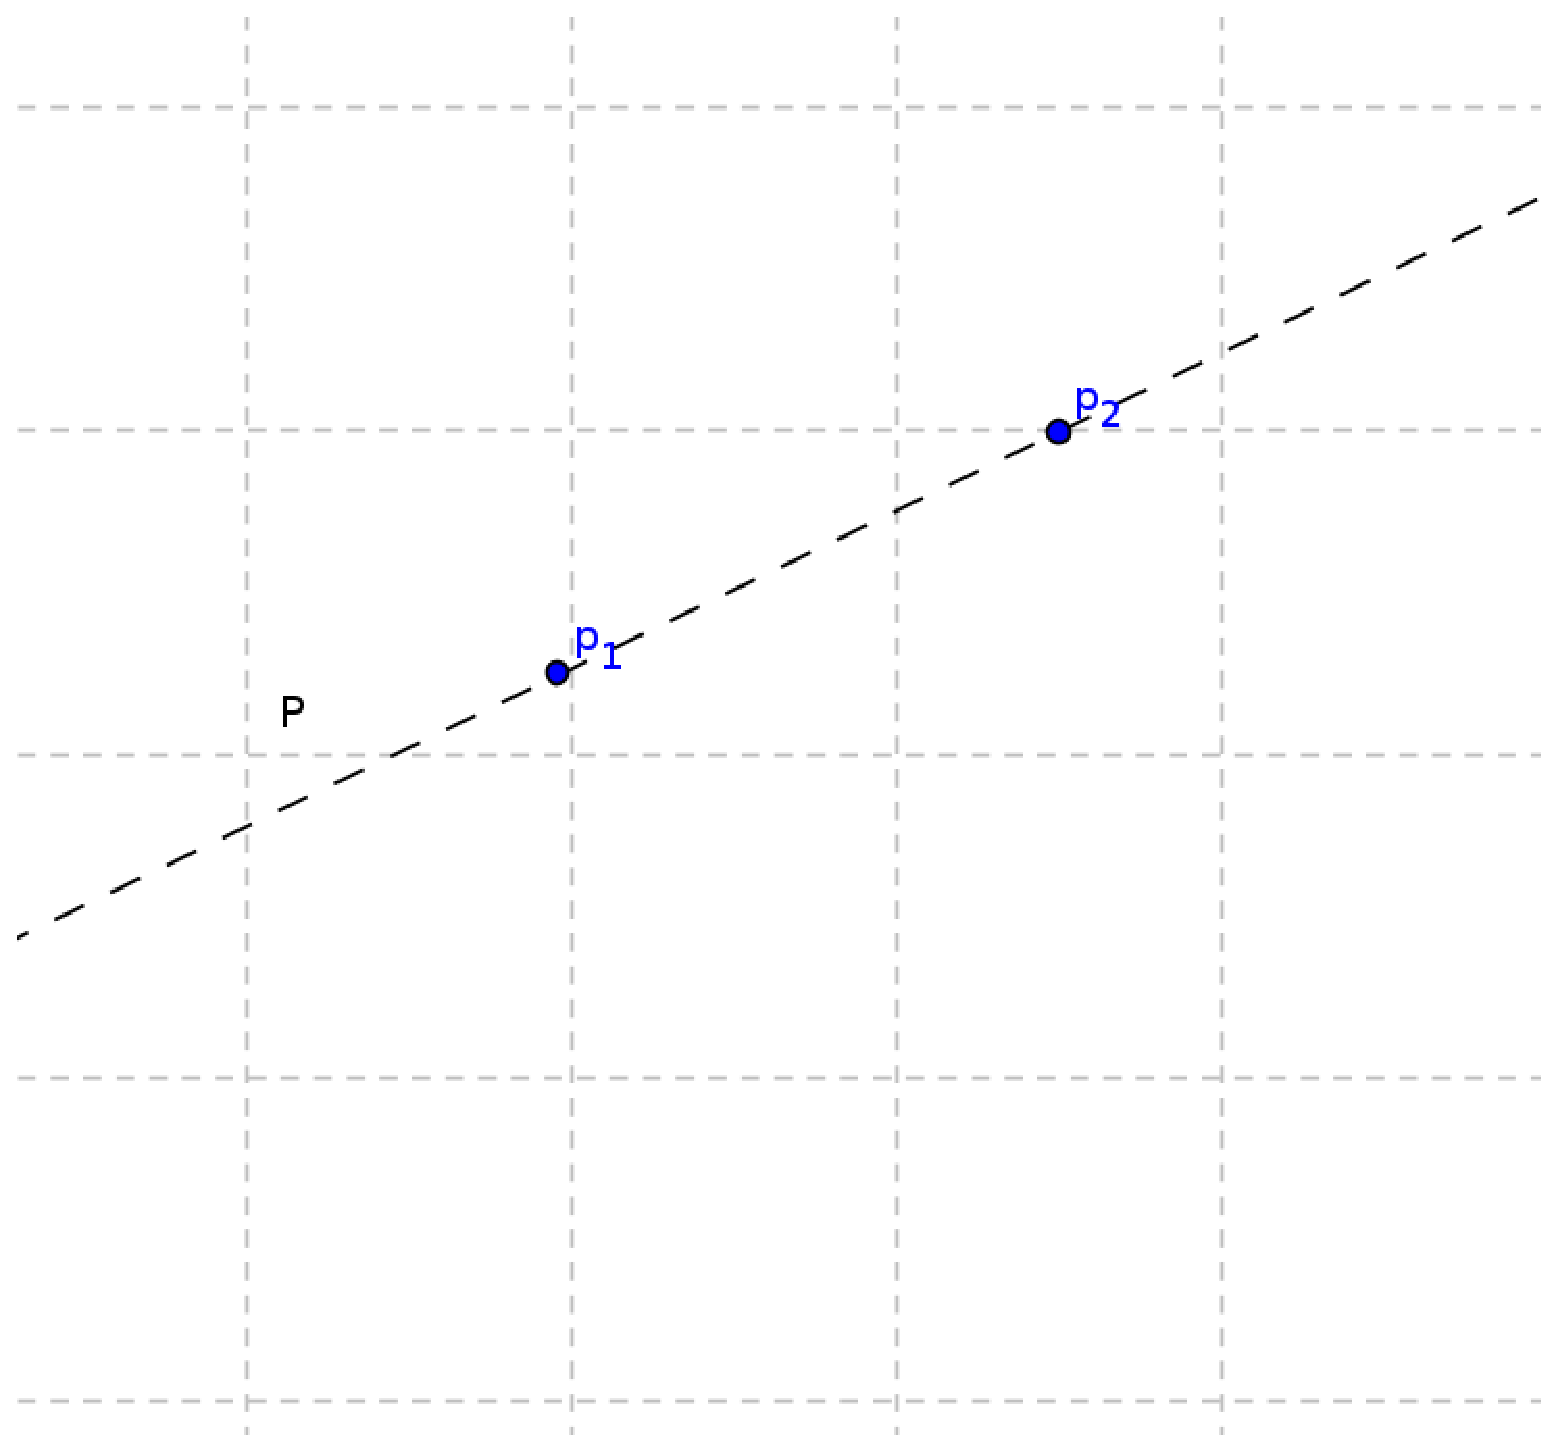
\includegraphics[height=130px]{media/Ax1.eps}
		    \end{center}
			\caption{Illustration de l'axiome 1}
		\end{figure}
		
		On peut ainsi construire les droites, comme avec une règle.
		\begin{axiome}
			Étant donné deux points $p_{1}$ et $p_{2}$ distincts, il existe un unique pli qui envoie $p_{1}$ sur $p_{2}$.
		\end{axiome}
		
		\begin{figure}
		    \begin{center}[h]
			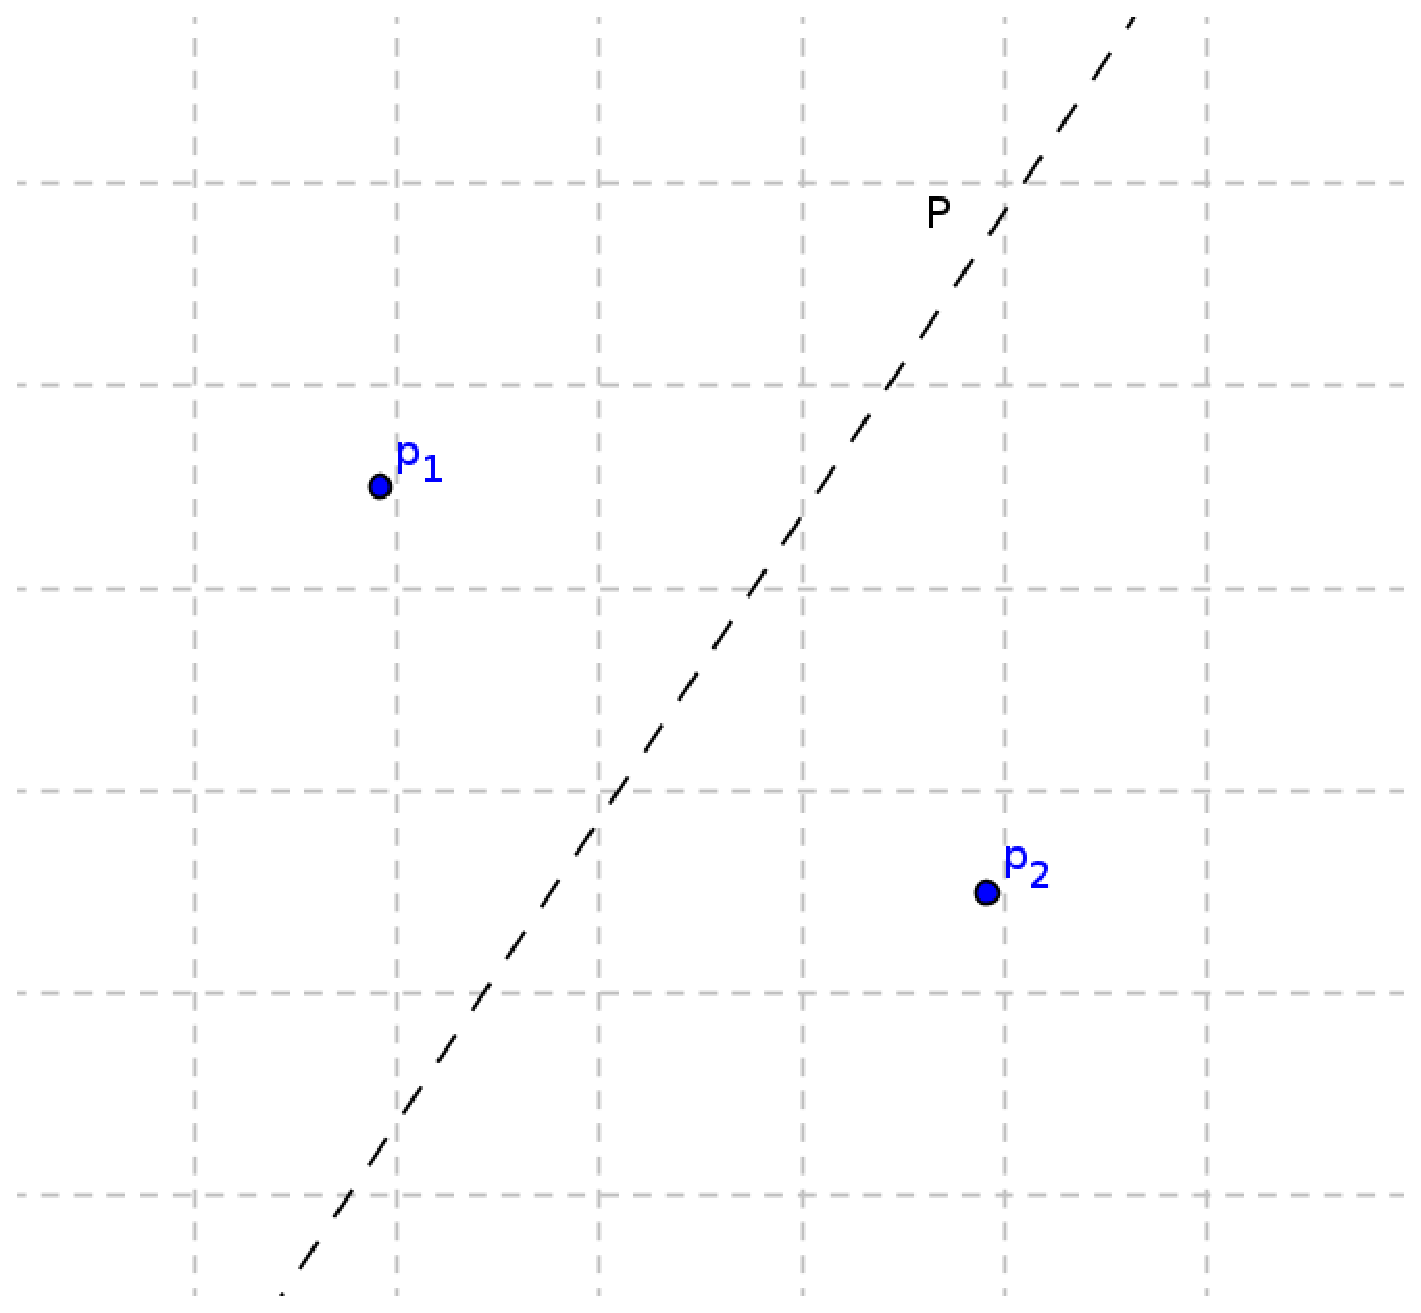
\includegraphics[height=130px]{media/Ax2.eps}
		    \end{center}
			\caption{Illustration de l'axiome 2}
		\end{figure}
		
		Cette opération est complétement équivalente au tracage d'une médiatrice entre deux points.
		\begin{axiome}
			Étant donné deux plis $P_{1}$ et $P_{2}$ distincts, il existe un unique pli qui envoie $P_{1}$ sur $P_{2}$.
		\end{axiome}
		
		\begin{figure}
		    \begin{center}[h]
			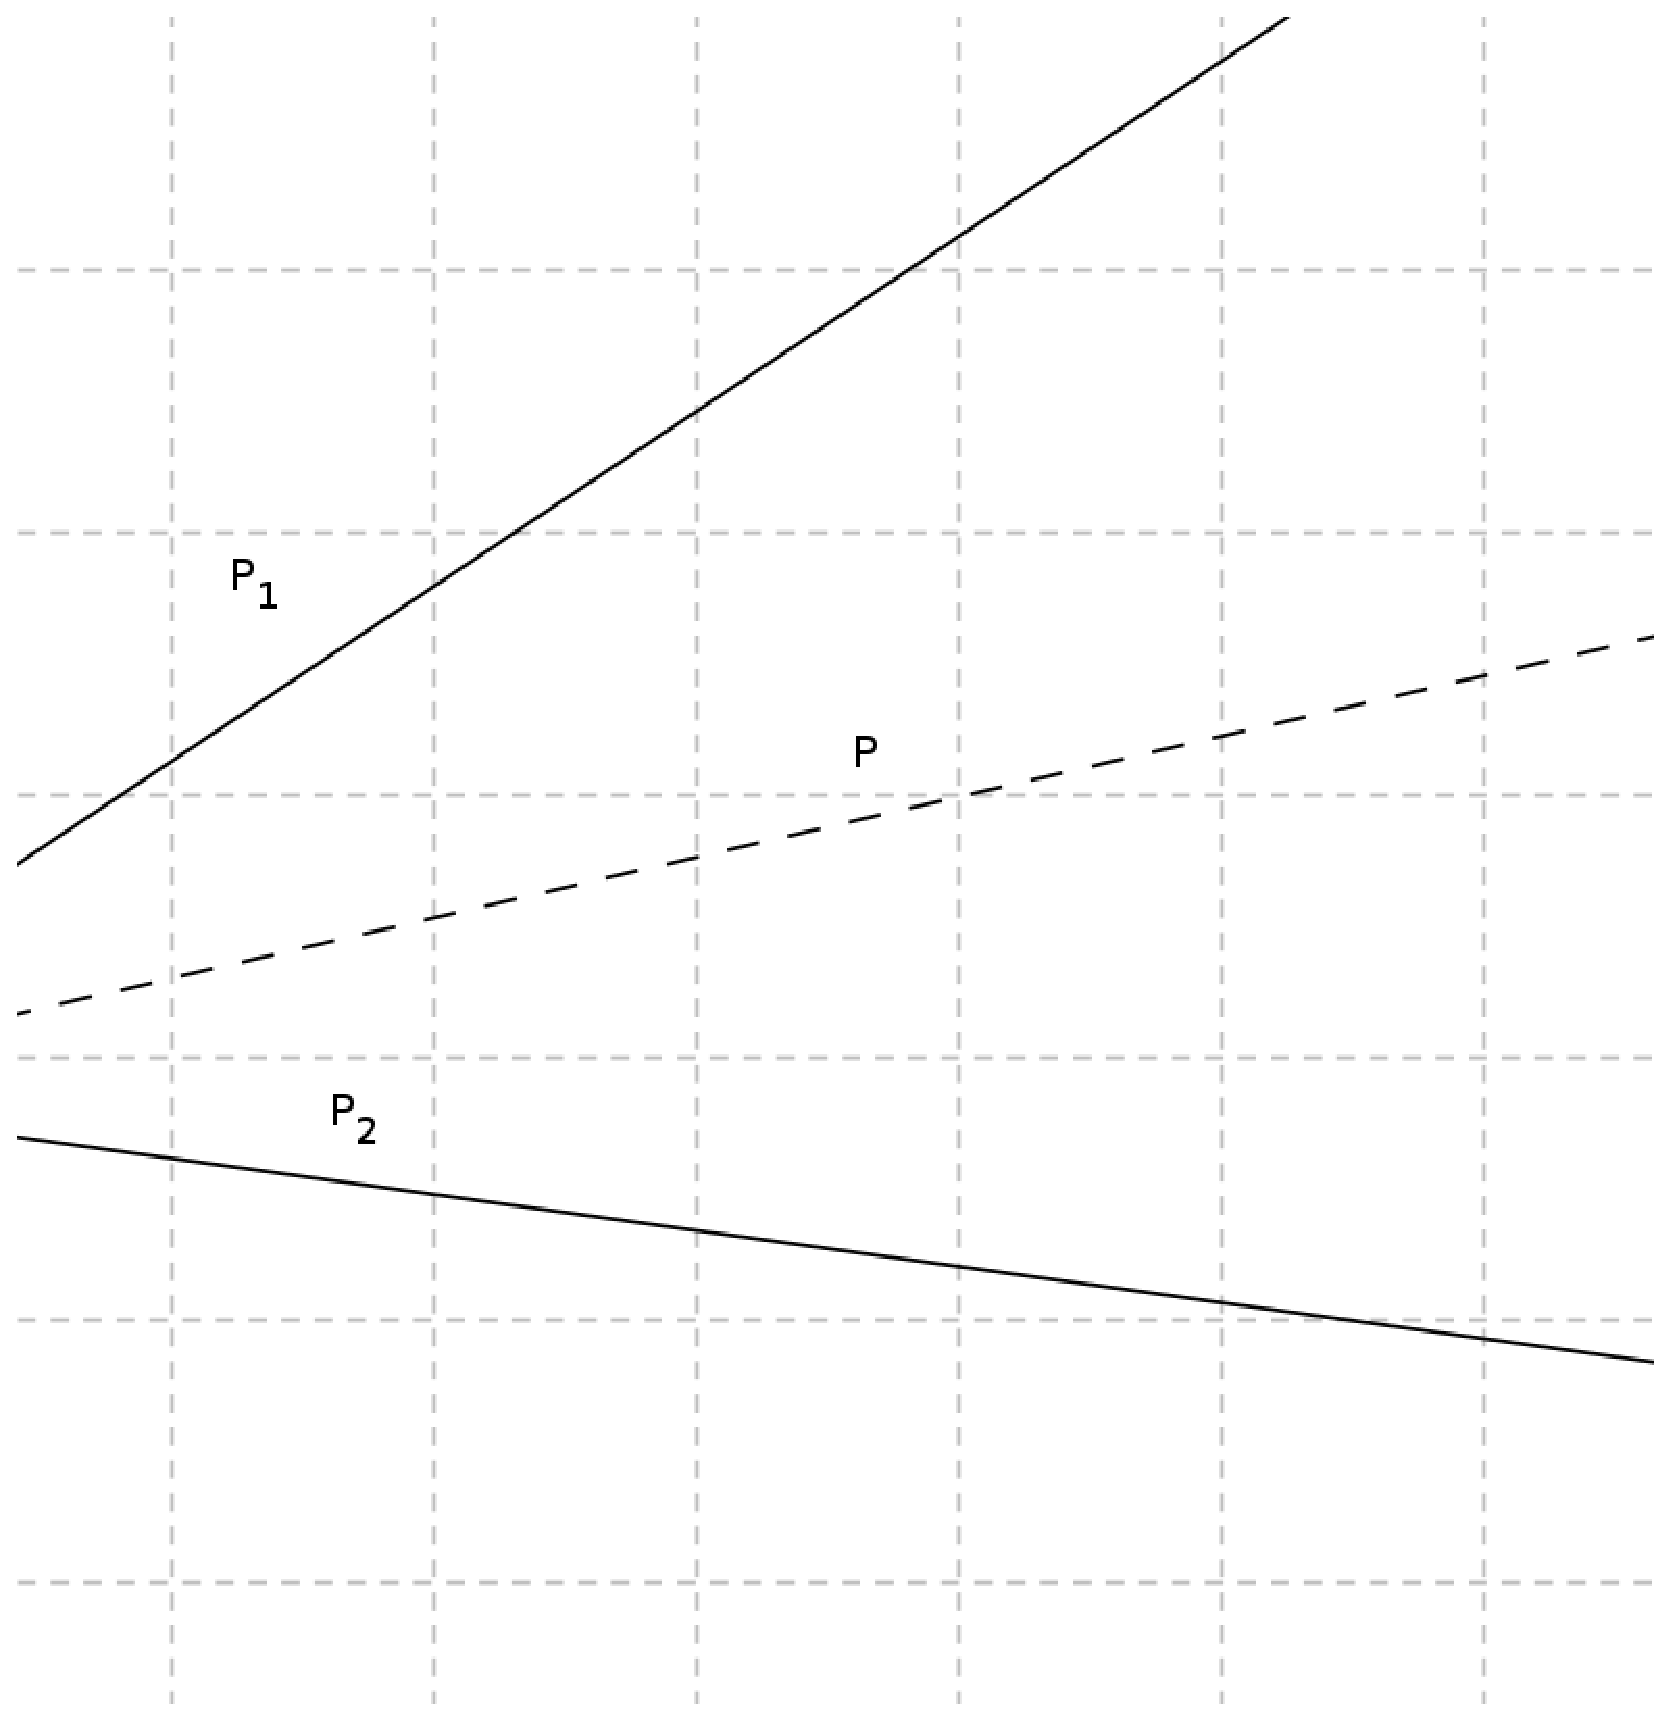
\includegraphics[height=130px]{media/Ax3.eps}
		    \end{center}
			\caption{Illustration de l'axiome 3}
		\end{figure}
		
		Cette opération est complétement équivalente au tracage d'une bissectrice entre deux droites.
		\begin{axiome}
			Étant donné un point $p_{1}$ et un pli $P_{1}$, il existe un unique pli $P$ qui passe par $p_{1}$ et soit perpendiculaire à $P_{1}$
		\end{axiome}
		
		\begin{figure}
		    \begin{center}[h]
			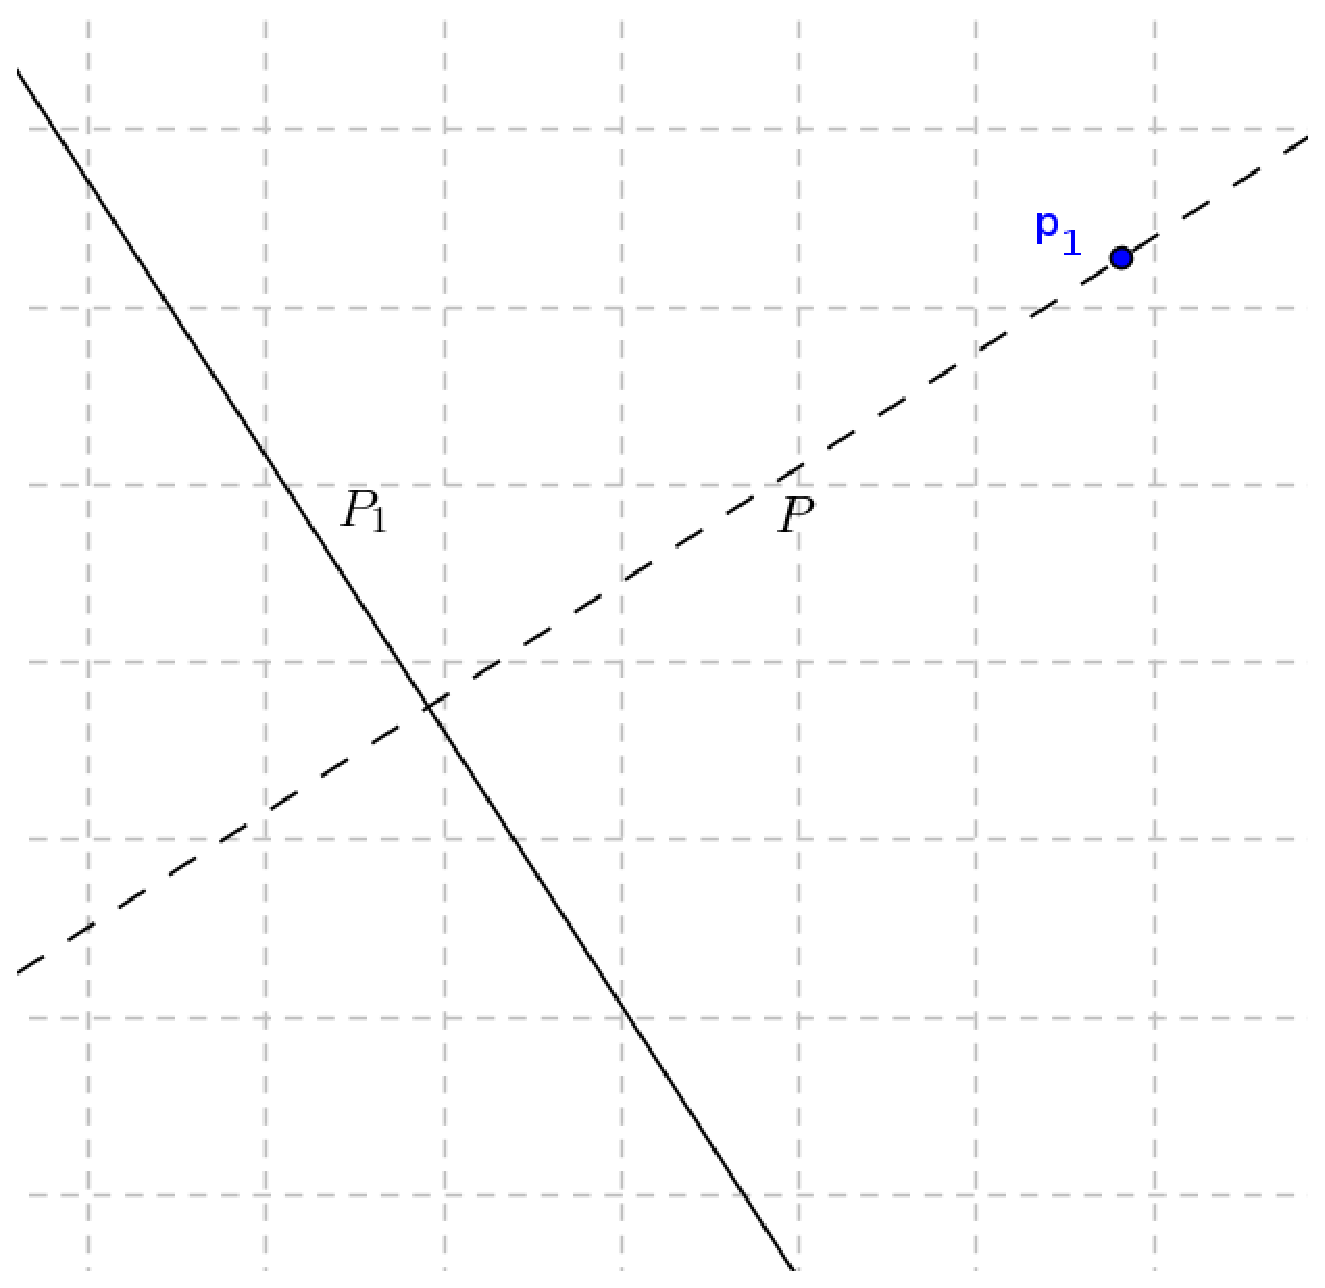
\includegraphics[height=130px]{media/Ax4.eps}
		    \end{center}
			\caption{Illustration de l'axiome 4}
		\end{figure}
		Cette opération est encore réalisable à la régle et au compas, moyennant la recherche de médiatrices.
		\begin{axiome}
			Étant donné deux points $p_{1}$ et $p_{2}$, et un pli $P_{1}$, il existe un pli $P$ qui envoie $p_{1}$ sur un point de $P_{1}$, en passant par $p_{2}$
		\end{axiome}
		\begin{figure}[h]
		    \begin{center}
			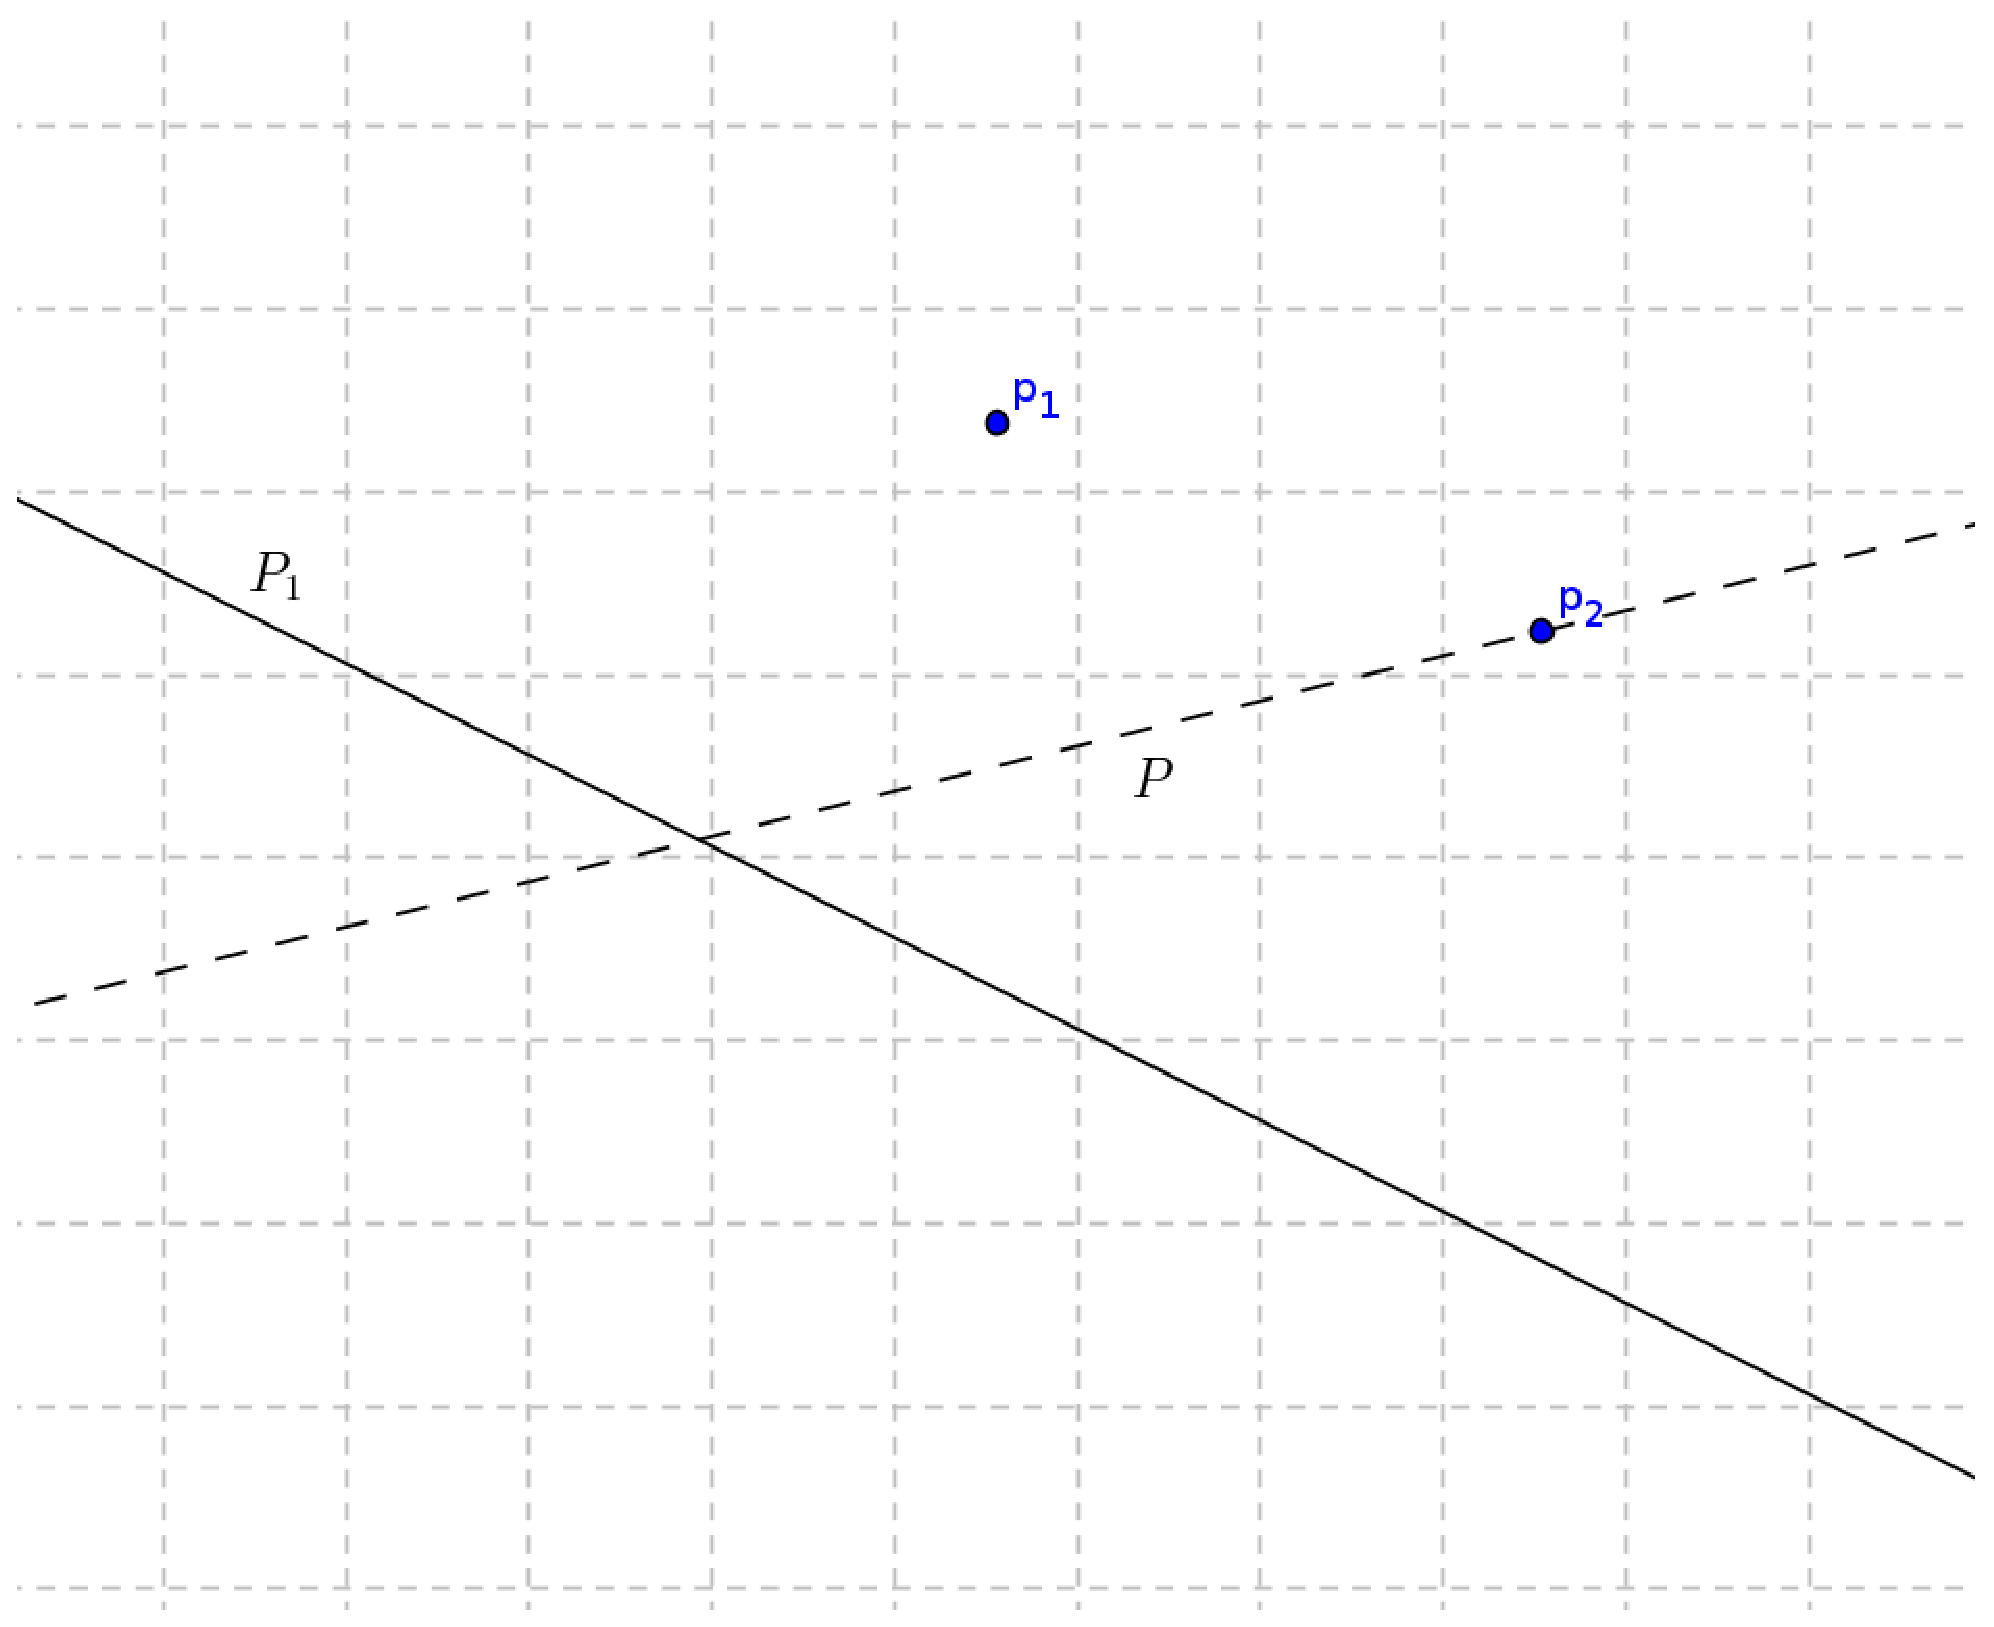
\includegraphics[height=130px]{media/Ax5.eps}
		    \end{center}
			\caption{Illustration de l'axiome 5}
		\end{figure}
		Cette opération correspond à la recherche d'une intersection entre un cercle et une droite. Il peut y avoir 0,1 ou 2 solutions.
		
		
		\begin{axiome}
			Étant donné deux points $p_{1}$ et $p_{2}$, et deux plis $P_{1}$ et $P_{2}$, il existe un pli $P$ qui envoie $p_{1}$ sur un point de $P_{1}$ et $p_{2}$ sur un point de $P_{2}$
		\end{axiome}
		\begin{figure}[h]
		    \begin{center}
			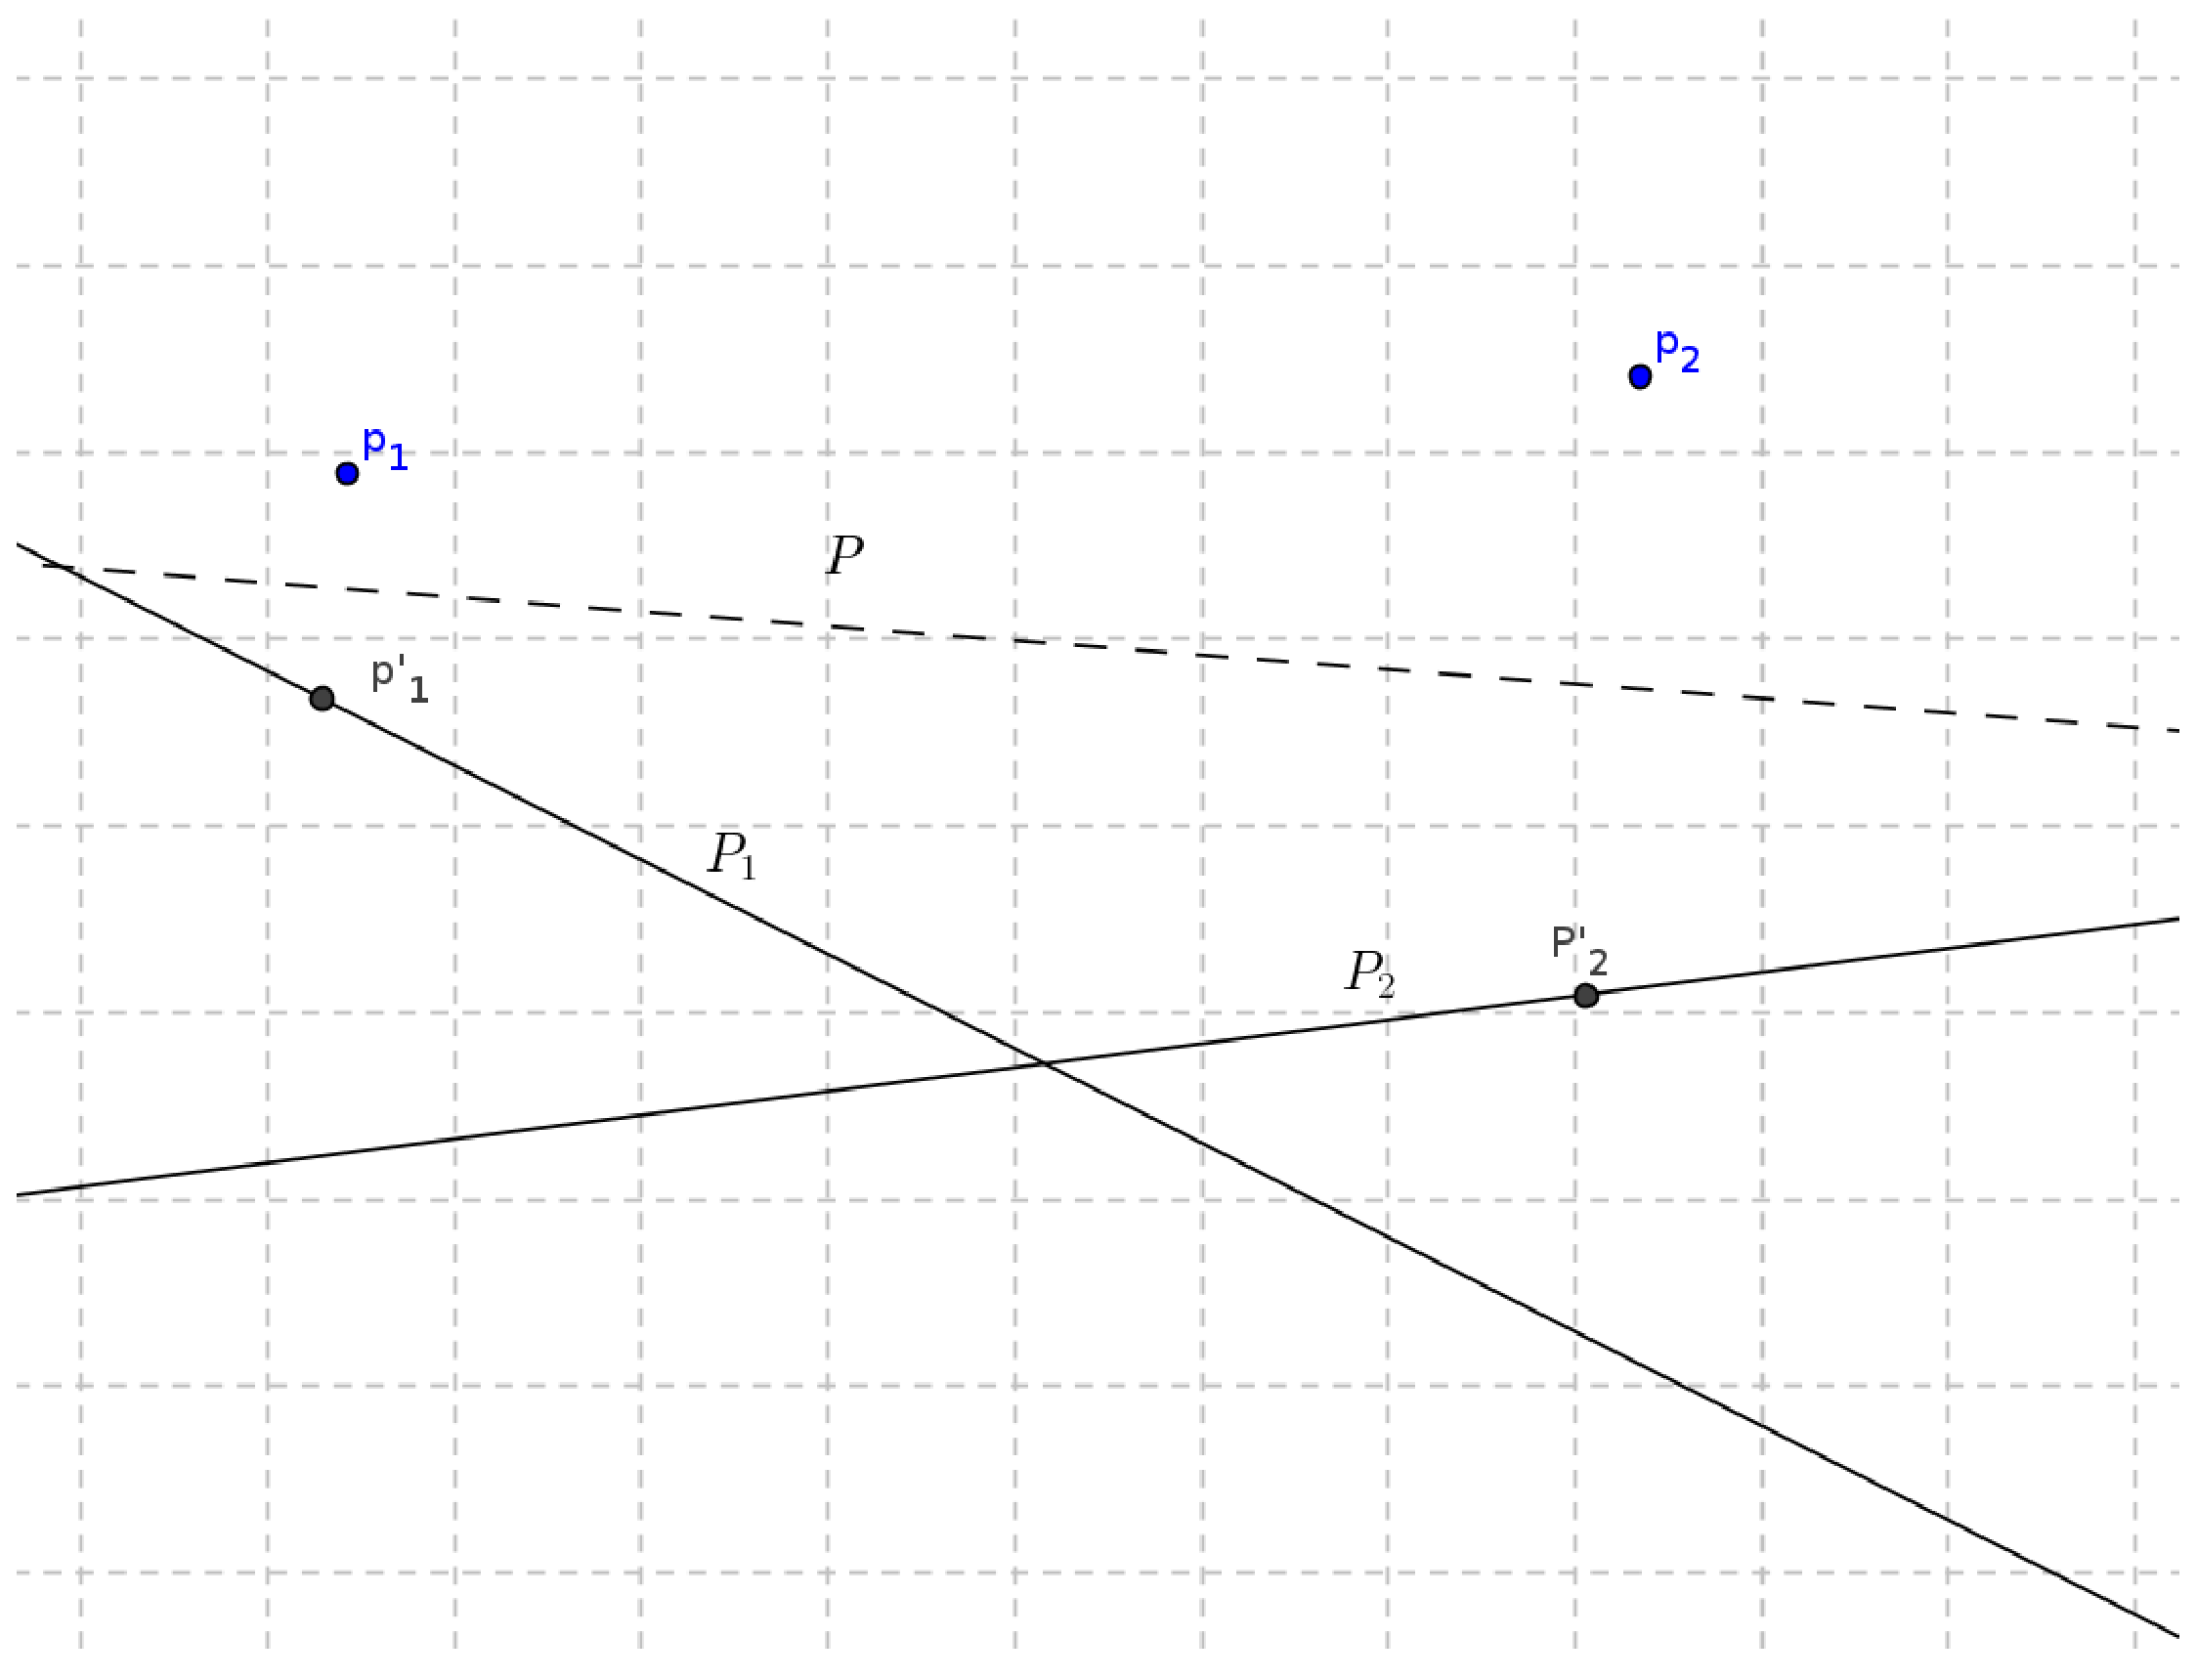
\includegraphics[height=130px]{media/Ax6.eps}
		    \end{center}
			\caption{Illustration de l'axiome 6}
		\end{figure}
		 C'est cette opération précise qui apporte un avantage au système axiomatique de l'origami. En effet on montrera par la suite qu'elle permet de résoudre des équations de degré 3.
		
		
		\begin{axiome}
			Étant donné un point $p_{1}$ et deux plis $P_{1}$ et $P_{2}$, il existe un pli qui envoie $p_{1}$ sur $P_{1}$, perpendiculairement à $P_{2}$
		\end{axiome}
		\begin{figure}[h]
		    \begin{center}
			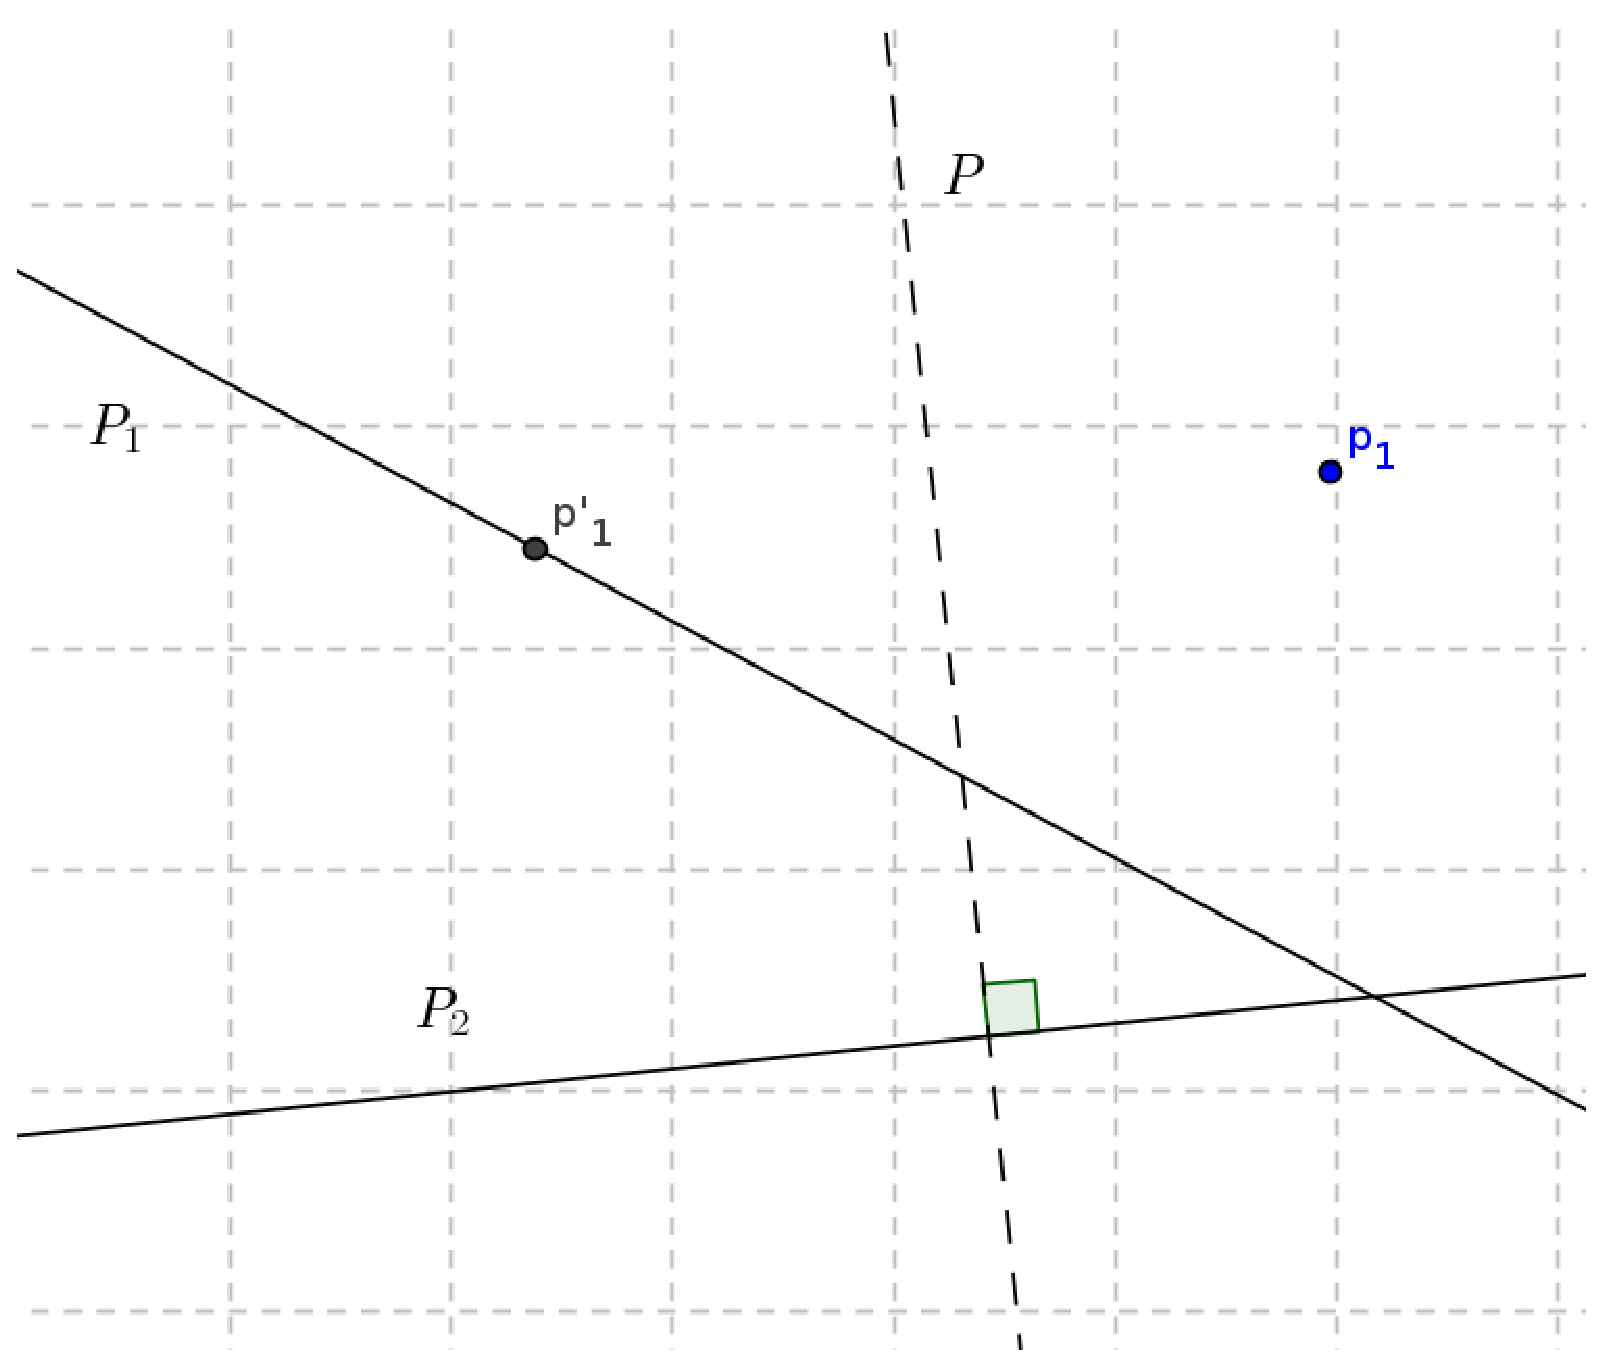
\includegraphics[height=130px]{media/Ax7.eps}
		    \end{center}
			\caption{Illustration de l'axiome 7}
		\end{figure}

\end{document}
